\section{Shape reconstruction}

\begin{theorem}
    A projective transformation $H$ that maps the circular points $I$ and $J$ onto themselves implies that $H$ is a similarity transformation. 
\end{theorem}
\begin{proof}
    When we multiply a similarity matrix $H_S$ by the circular point $I$, we obtain a multiple of $I$.
    Similarly, the same result is obtained for the other circular point, $J$.
\end{proof}
The given image represents a general projective mapping of the original scene. 
Consequently, the image of the circular points, denoted as $(I^{'},J^{'})$, differs from $I$ and $J$. 
To utilize $I^{'},J^{'}$ as additional information, we apply a new projective mapping $H_{SR}$ to map $I^{'},J^{'}$ back to $I,J$. 
This process generates a new modified image where the circular points $I,J$ are restored.
As per the theorem, the obtained model (new image) is similar to the original scene, representing a shape reconstruction of the scene.
\begin{figure}[H]
    \centering
    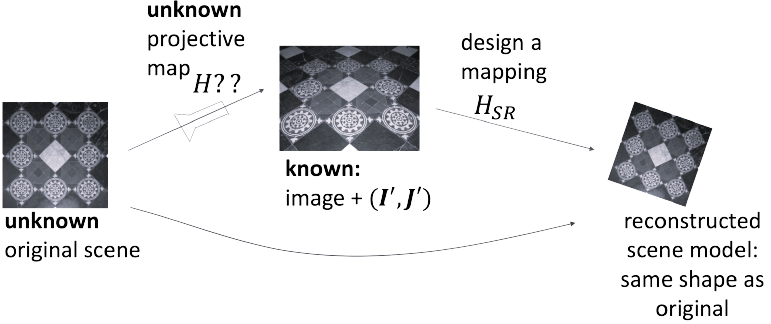
\includegraphics[width=0.75\linewidth]{images/HSR.png}
\end{figure}
The method comes with certain challenges:
\begin{itemize}
    \item Finding a projective mapping $H_{SR}$ that restores $I^{'},J^{'}$ to $I,J$. 
    \item Determining the vanishing line.
\end{itemize}

\subsection*{Identify a projective transformation}
Discovering a projective transformation $H_{SR}$ that restores $I^{'}, J^{'}$ to $I, J$ is equivalent to finding one of the $\infty^{4}$ matrices that satisfy:
\[\begin{cases}
    H_{SR}I^{'}=I \\
    H_{SR}J^{'}=J
\end{cases}\]
This task can be quite challenging.

Let's utilize alternative information: the degenerate conic dual to $I^{'},J^{'}$, represented as $C_{\infty}^{'*}=I^{'}J^{'T}+J^{'}I^{'T}$, which corresponds to the image of the original conic dual to the circular points $(I,J)$, expressed as: 
\[C_{\infty}^{*}=IJ^{T}+JI^{T}\]
Since $(I^{'},J^{'})$ is the image of $(I,J)$, then also $C_{\infty}^{'*}$ is the image of $C_{\infty}^{*}$. 
As a result, any projective transformation $H_{SR}$ that restores $(I^{'},J^{'})$ to $(I,J)$ also restores $C_{\infty}^{'*}$ to $C_{\infty}^{*}$. 
By applying the transformation rule for dual conics under projective mappings, we get:
\[C^{*}_{\infty}=H_{SR}C^{'*}_{\infty}H_{SR}^T\]
Reversing this relationship, we find:
\[C_{\infty}^{'*}=H_{SR}^{-1} 
\begin{bmatrix}
    1 & 0 & 0 \\
    0 & 1 & 0 \\
    0 & 0 & 0
\end{bmatrix}
H_{SR}^{-T}\]
Applying singular value decomposition (SVD) to this equation, we find that the matrices $H_{SR}^{-1}$ and $H_{SR}^{-T}$ are orthogonal. 
Consequently, we have:
\[\textnormal{SVD}(C_{\infty}^{'*})=U_\perp
\begin{bmatrix}
    1 & 0 & 0 \\
    0 & 1 & 0 \\
    0 & 0 & 0
\end{bmatrix}
U_{\perp}^T\]
Which provides a unique solution: $H_{SR}=U_{\perp}^{-1}=U_{\perp}^T$. 
To address the issues with image rectification, we need to modify the matrix $H_{SR}$ as follows:
\[H_{SR}=
\begin{bmatrix}
    \frac{1}{\sqrt{a}} & 0 & 0 \\
    0 & \frac{1}{\sqrt{b}} & 0 \\
    0 & 0 & 1
\end{bmatrix}
U^T
\]

\subsection*{Determine the vanishing line}
To determine the vanishing line, one can leverage additional information from the observed scene. 
This information can be used to establish the following constraints:
\begin{enumerate}
    \item Known angles between lines: when the angles between lines in the scene are known, these angles can be used to constrain the vanishing line. 
        The angle between two lines is related to the angle between their normal directions and is independent of parameters $c_1$ and $c_2$. 
        Mathematically, this relationship is expressed as:
        \[\cos\vartheta=\dfrac{a_1a_2+b_1b_2}{\sqrt{(a_1^2+b_1^2)(a_2^2+b_2^2)}}\]
        Here, $a_1$, $b_1$, $a_2$, and $b_2$ are coefficients of the normal vectors of the lines. 
        By rewriting the terms, this equation can be expressed as: 
        \[\cos\vartheta=\dfrac{l^TC_{\infty}^{*}m}{\sqrt{(l^TC_{\infty}^{*}l)(m^TC_{\infty}^{*}m)}}\]
        This equation can be further simplified by using the rules obtaining $C_{\infty}^{*}=H^{-1}C_{\infty}^{*'}H^{-T}$.  
        Now, we can rewrite $l^TC_{\infty}^{*}m$ as $l^{'T}C_{\infty}^{*'}m^{'}$. 
        With these transformations, the equation becomes:
        \[\cos\vartheta=\dfrac{l^{'T}C_{\infty}^{*'}m^{'}}{(l^{'T}C_{\infty}^{*'}l^{'})(m^{'T}C_{\infty}^{*'}m^{'})}\]
        In this case, $m^{'}$ and $l^{'}$ are obtained from the image. 
        Since the angle is known, this equation provides a linear constraint on $C_{\infty}^{*'}$, that is linear when the lines are perpendicular ($\cos\vartheta=0$).
        The unknown matrix $C_{\infty}^{'}$ is symmetric, homogeneous, and singular, providing four independent constraints.
    \item Known shape of objects: if the shape of objects in the scene is known, the reconstruction matrix $H_{SR}$ can be determined. 
        The transformation matrix is defined as:
        \[H_{SR}=
        \begin{bmatrix}
            \frac{1}{\sqrt{a}} & 0 & 0 \\
            0 & \frac{1}{\sqrt{b}} & 0 \\
            0 & 0 & 1
        \end{bmatrix}
        U^T
        \]
        The Euclidean reconstructed image is calculated as $M_S=H_{SR} \cdot \textnormal{image}$
    \item Combinations of constraints: it is also possible to use a combination of known angles between lines and the shape of objects for additional constraints.
    \item Observation of rigid planar motion: when observing rigid planar motion, which is a similarity transformation, the circular points remain invariant.
        The object has three degrees of freedom, and the center of rotation and the rotation angle can be determined.
        Given a matrix $H$, the eigenvectors of $H$ correspond to fixed points, and the eigenvectors of $H^{-T}$ correspond to fixed lines of the transformation.
        The eigenvectors can be used to extract important information:
        \begin{itemize}
            \item Eigenvectors $I^{'},J^{'}$ correspond to complex eigenvalues. 
            \item The phase of these eigenvectors is the rotation angle.
            \item Eigenvector $O^{'}$ correspond to real eigenvalues. 
        \end{itemize}
        The three eigenvectors of $H$ are proportional to three distinct values: 1, $e^{i\theta}$, and $-e^{i\theta}$.
        The eigenvector corresponding to the eigenvalue 1 represents the image of the center of rotation, denoted as $O$, and the angle $\theta$ corresponds to the rotation angle. 
        The eigenvectors associated with the complex eigenvalues represent the images of the circular points $I^{'},J^{'}$. 
        Therefore, using the relationship $C_{\infty}^{'*}=I^{'}J^{'T}+J^{'}I^{'T}$, the singular value decomposition can be applied to obtain $\textnormal{SVD}(C_{\infty}^{'*})=UC_{\infty}^{*}U^T$, where $U^T$ is the rectification matrix. 
        Two methods can be used to address this:
        \begin{itemize}
            \item Direct method: 
                \begin{enumerate}
                    \item Find $C_{\infty}^{*'}$. 
                    \item Compute $H_{rect}$ for rectification. 
                \end{enumerate}
            \item Stratified method: 
                \begin{enumerate}
                    \item Perform affine reconstruction from projective to affine.
                    \item Perform shape reconstruction from affine to metric.
                \end{enumerate}
        \end{itemize}
        In some cases, the stratified method reduces numerical errors, providing a more accurate result.
\end{enumerate}